\ifx\wholebook\relax \else

\documentclass[b5paper]{article}
\usepackage[nomarginpar
  %, margin=.5in
]{geometry}

\addtolength{\oddsidemargin}{-0.05in}
\addtolength{\evensidemargin}{-0.05in}
\addtolength{\textwidth}{0.1in}

\usepackage[en]{../../../prelude}

\setcounter{page}{1}

\begin{document}

\title{Binary Search Tree}

\author{Xinyu LIU
\thanks{{\bfseries Xinyu LIU} \newline
  Email: liuxinyu95@gmail.com \newline}
  }

\maketitle
\fi

\markboth{Binary search tree}{Elementary Algorithms}

\ifx\wholebook\relax
\chapter{Binary Search Tree}
\numberwithin{Exercise}{chapter}
\fi

Array and list are typically considered the basic data structures. However, we'll see they are not necessarily easy to implement in chapter 12. Upon imperative settings, array is the most elementary data structures. It is possible to implement linked-list using arrays (\cref{sec:list-index-array}). While in functional settings, linked-list acts as the building blocks to create array and other data structures. The binary search trees is another basic data structure. Jon Bentley gives a problem in {\em Programming Pearls}\cite{Bentley}: how to count the number of word occurrences in a text. Here is a solution:\index{word counter}

\lstset{frame=single}
\begin{lstlisting}[language=Bourbaki]
void wordCount(Input in) {
    Map<String, Int> map
    while String w = read(in) {
        map[w] = if map[w] == null then 1 else map[w] + 1
    }
    for var (w, c) in map {
        print(w, ":", c)
    }
}
\end{lstlisting}

\section{Definition}
\label{introduction} \index{binary tree}

The \texttt{map} is a binary search tree. Here we use the word as the key, and its occurrence number as the value. This program is a typical application of binary search tree. Let us firstly define the {\em binary tree}. A binary tree is either empty ($\nil$)\footnote{The great mathematician André Weil invented this symbol for null set. It comes from the Norwegian alphabet.}; or contains 3 parts: an element $k$, and two sub-trees called left($l$) and right($r$) children, denoted as $(l, k, r)$. A none empty binary tree consists of multiple nodes, each is either empty or stores the element of type $K$. We define the type of the binary tree as $Tree\ K$. We say a node is a leaf if both sub-trees are empty, or it's a branch node.

\begin{figure}[htbp]
  \centering
  \subcaptionbox{Binary tree structure}{\includegraphics[scale=0.4]{img/lvr}} \\
  \subcaptionbox{A binary tree}{\includegraphics[scale=0.35]{img/btexample}}
  \caption{Binary tree}
  \label{fig:binary-tree-example}
\end{figure}

\index{binary search tree}
A binary search tree is a special binary tree that its elements are comparable\footnote{It is abstract ordering, not limit to magnitude, but like precedence, subset of etc. the `less than' (<) is abstract.}, and satisfies: for any non empty node $(l, k, r)$, all the keys in the left sub-tree $< k$; $k <$ any key in the right sub-tree. \Cref{fig:bst-example} shows an example of binary search tree. Comparing with \cref{fig:binary-tree-example}, we can see the differences in ordering. For this reason, we call the comparable element as {\em key}, and the augmented data as {\em value}. The type is $Tree\ (K, V)$.

\begin{figure}[htbp]
  \begin{center}
   \includegraphics[scale=0.35]{img/bst-1}
   \caption{A binary search tree} \label{fig:bst-example}
  \end{center}
\end{figure}

\index{binary search tree!data layout}
\Cref{fig:node-layout-parent} shows the data layout. A node contains a key, a value (optional), left, right sub-tree references, and a parent reference for easy backtracking. When the context is clear, we skip the value (augmented data). The appendix of this chapter includes an example definition. We needn't reference for backtracking in functional settings, but use top-down recursive computation. Below is the example functional definition:


\begin{figure}[htbp]
  \begin{center}
   \includegraphics[scale=0.5]{img/node-layout-parent}
   \caption{Node layout with parent reference.} \label{fig:node-layout-parent}
  \end{center}
\end{figure}

\begin{Haskell}
data Tree a = Empty | Node (Tree a) a (Tree a)
\end{Haskell}

\section{Insert}
\index{binary search tree!insert}

When insert a key $k$ (with the value) to the binary search tree $T$, we need maintain the ordering. If the tree is empty, create a leaf of $k$. Otherwise, let the tree be $(l, x, r)$. If $k < x$, insert it to the left sub-tree $l$; otherwise, insert to the right $r$. If $k = x$, it already exists in the tree. We overwrite the value (update). Alternatively, we cab append the data or do nothing. We skip this case. Below is the recursive definition and example program:

\be
\begin{array}{rcl}
insert\ k\ \nil & = & (\nil, k, \nil) \\
insert\ k\ (l, x, r) & = & \begin{cases}
  k < x: & (insert\ k\ l, x, r) \\
  \text{otherwise}: & (l, x, insert\ k\ r) \\
  \end{cases}
\end{array}
\ee

\begin{Haskell}
insert k Empty = Node Empty k Empty
insert k (Node l x r) | k < x = Node (insert k l) x r
                      | otherwise = Node l x (insert k r)
\end{Haskell}

This implementation uses the {\em pattern matching} feature. We give another example without pattern matching in the appendix. We can eliminate the recursion with iterative loops:

\begin{algorithmic}[1]
\Function{Insert}{$T, k$}
  \State $root \gets T$
  \State $x \gets$ \Call{Create-Leaf}{$k$}
  \State $parent \gets$ NIL
  \While{$T \neq$ NIL}
    \State $parent \gets T$
    \If{$k <$ \Call{Key}{$T$}}
      \State $T \gets $ \Call{Left}{$T$}
    \Else
      \State $T \gets $ \Call{Right}{$T$}
    \EndIf
  \EndWhile
  \State \Call{Parent}{$x$} $\gets parent$
  \If{$parent = $ NIL} \Comment{$T$ in empty}
    \State \Return $x$
  \ElsIf{$k <$ \Call{Key}{$parent$}}
    \State \Call{Left}{$parent$} $\gets x$
  \Else
    \State \Call{Right}{$parent$} $\gets x$
  \EndIf
  \State \Return $root$
\EndFunction
\Statex
\Function{Create-Leaf}{k}
  \State $x \gets $ \Call{Empty-Node}{}
  \State \Call{Key}{$x$} $ \gets k$
  \State \Call{Left}{$x$} $ \gets $ NIL
  \State \Call{Right}{$x$} $ \gets $ NIL
  \State \Call{Parent}{$x$} $ \gets $ NIL
  \State \Return $x$
\EndFunction
\end{algorithmic}

Where \textproc{Key}($T$) accesses the key of the node:

\be
\begin{array}{rcl}
key\ \nil & = & \textit{Nothing} \\
key\ (l, k, r) & = & \textit{Just}\ k \\
\end{array}
\ee

We can repeat insert every element from a list, convert the list to a binary search tree:

\[
\begin{array}{rcl}
\textit{fromList}\ [\ ] & = & \nil \\
\textit{fromList}\ (x \cons xs) & = & insert\ x\ (\textit{fromList}\ xs) \\
\end{array}
\]

Or define it with fold (chapter 1) in Curried form: \textit{fromList} = $foldr\ insert\ \nil$. We arrange the input arguments in symmetric order: $insert\ k\ t$ and \textproc{Insert}($T, k$) for functional and imperative implementations. Such that to use $foldr$ for the former, and $foldl$ (or for-loop) for the latter:

\begin{algorithmic}[1]
\Function{From-List}{$X$}
  \State $T \gets $ NIL
  \For{each $x$ in $X$}
    \State $T \gets$ \Call{Insert}{$T, x$}
  \EndFor
  \State \Return $T$
\EndFunction
\end{algorithmic}

\section{Traverse}
\index{binary search tree!traverse}

Traverse is to visit every element in the binary search tree. There are 3 ways: pre-order, in-order, and post-order tree walk. They are named to highlight the order of visiting key between/before/after sub-trees.

\begin{itemize}
\item pre-order: \textbf{key} - left - right;
\item in-order: left - \textbf{key} - right;
\item post-order: left - right - \textbf{key}.
\end{itemize}

\index{pre-order traverse} \index{in-order traverse} \index{post-order traverse}

The `visit' is recursive. For the tree in \cref{fig:bst-example}, the corresponding visiting orders are as below:

\begin{itemize}
\item pre-order: 4, 3, 1, 2, 8, 7, 16, 10, 9, 14
\item in-order: 1, 2, 3, 4, 7, 8, 9, 10, 14, 16
\item post-order: 2, 1, 3, 7, 9, 14, 10, 16, 8, 4
\end{itemize}

It is not by accident that the in-order traverse gives an ascending list, but is guaranteed by the definition of the binary search tree (see exercise \label{ex:BST-in-order-sort}). Define $map$ that in-order traverses and applies function $f$ to every element of the tree. It transforms a tree to another tree of the same structure (isomorphic).

\be
\begin{array}{rcl}
map\ f\ \nil & = & \nil \\
map\ f\ (l, k, r) & = & (map\ f\ l, f\ k, map\ f\ r)
\end{array}
\ee

If we only need manipulate keys but not transform the tree, we can implement in-order traverse as below:

\begin{algorithmic}[1]
\Function{Traverse}{$T, f$}
  \If{$T \neq$ NIL}
    \State \textproc{Traverse}(\Call{Left}{$T$}, $f$)
    \State $f$(\Call{Key}{$T$})
    \State \textproc{Traverse}(\Call{Right}{$T$, $f$})
  \EndIf
\EndFunction
\end{algorithmic}

We can change the $map$ function, convert a binary search tree to a sorted list.

\be
\begin{array}{rcl}
toList\ \nil & = & [\ ] \\
toList\ (l, k, r) & = & toList\ l \doubleplus [k] \doubleplus toList\ r \\
\end{array}
\ee

We can develop a sort algorithm: convert a list to a binary search tree, then convert the tree back to ordered list, namely `tree sort': $sort\ X = toList\ (\textit{fromList}\ X)$, or write as function composition\cite{func-composition}:

\be
  sort = toList \circ \textit{fromList}
\ee

We define the generic fold for binary trees (see chapter 1 for fold):

\be
\begin{array}{rcl}
foldt\ f\ g\ z\ \nil & = & z \\
foldt\ f\ g\ z\ (l, k, r) & = & g\ (foldt\ f\ g\ z\ l)\ (f\ k)\ (foldt\ f\ g\ z\ r) \\
\end{array}
\ee

Where $f: A \to B$, sends the key $k$ of type $A$ in the tree to $m = f(k)$ of type $B$. It recursively folds the left and right sub-trees (from $z$) to get $x$ and $y$ respectively, then combines the three things together as $g\ x\ m\ y$. We can define $map$ with $foldt$:

\be
map\ f = foldt\ f\ (x\ m\ y\ \mapsto (x, m, y))\ \nil
\ee

$foldt$ preserves the tree structure with the ternary function $g$. If don't care about the tree structure, we can use a binary function $f : A \times B \to B$ to simplify, fold a tree of type $Tree\ A$ to a value of type $B$:

\be
\begin{array}{rcl}
fold\ f\ z\ \nil & = & z \\
fold\ f\ z\ (l, k, r) & = & fold\ f\ (f\ k\ (fold\ f\ z\ r))\ l\\
\end{array}
\ee

For example: $sum = fold\ (+)\ 0$ sums all elements of the tree; $length = fold\ (x\ n \mapsto n + 1)\ 0$ counts the number of elements in the tree. However, $fold$ can not define $map$, as the binary function $f$ loss the tree structure.

\begin{Exercise}\label{ex:bst-traverse}
\index{tree reconstruction}
\Question{Given the in-order and pre-order traverse results, rebuild the tree, and output the post-order traverse result. For example:
  \begin{itemize}
  \item Pre-order: 1, 2, 4, 3, 5, 6;
  \item In-order: 4, 2, 1, 5, 3, 6;
  \item Post-order: ?
  \end{itemize}
}

\Question{Write a program to rebuild the binary tree from the pre-order and in-order traverse lists.}

\Question{For binary search tree, prove that the in-order traverse always gives ordered list.
\label{ex:BST-in-order-sort}
}

\Question{What is its complexity of tree sort for $n$ elements?}

\Question{Define $toList$ with fold.}

\Question{Define $depth\ t$ with folding, to calculate the height of a binary tree.}
\end{Exercise}

\begin{Answer}[ref={ex:bst-traverse}]
\Question{Given the in-order and pre-order traverse results, rebuild the tree, and output the post-order traverse result. For example:

  \begin{itemize}
  \item Pre-order: 1, 2, 4, 3, 5, 6;
  \item In-order: 4, 2, 1, 5, 3, 6;
  \item Post-order: ?
  \end{itemize}

[4, 2, 5, 6, 3, 1]
}

\Question{Write a program to rebuild the binary tree from the pre-order and in-order traverse lists.

\vspace{3mm}
Let $P$ be the pre-order traverse result, $I$ be the in-order result. If$P = I = [\ ]$, then the binary tree is empty $\nil$. Otherwise, the pre-order is recursive `key - left - right', hence the first element $m$ in $P$ is the key of the root. The in-order is recursive `left - key - right', we can find $m$ in $I$, which splits $I$ into three parts: $[a_1, a_2, ..., a_{i-1}, m, a_{i+1}, a_{a+2}, ..., a_n]$. Let $I_l = I[1, i), I_r = I[i+1, n]$, where $[l, r)$ includes $l$, but excludes $r$. Either can be empty $[\ ]$. In these three parts $I_l, m, I_r$, $I_l$ is the in-order traverse result of the left sub-tree, $I_r$ is the in-order result of the right sub-tree. Let $k = |I_l|$ be the size of the left sub-tree, we can split $P[2, n]$ at $k$ to two parts: $P_l, P_r$, where $P_l$ contains the first $k$ elements. We next recursively rebuild the left sub-tree from $(P_l, I_l)$, rebuild the right sub-tree from $(P_r, I_r)$:

\[
\begin{array}{rcl}
\textit{rebuild}\ [\ ]\ [\ ] & = & \nil \\
\textit{rebuild}\ (m \cons ps)\ I & = & (\textit{rebuild}\ P_l\ I_l, m, \textit{rebuild}\ P_r\ I_r) \\
\end{array}
\]

Where:

\[
\begin{cases}
(I_l, I_r) & = \textit{splitWith}\ m\ I \\
(P_l, P_r) & = \textit{splitAt}\ |I_l|\ ps \\
\end{cases}
\]

Below is the example program:
\begin{Haskell}
rebuild [] _ = Empty
rebuild [c] _ = Node Empty c Empty
rebuild (x:xs) ins = Node (rebuild prl inl) x (rebuild prr inr) where
  (inl, _:inr) = (takeWhile (/= x) ins, dropWhile (/=x) ins)
  (prl, prr) = splitAt (length inl) xs
\end{Haskell}

We can also update the left and right boundary to implement:
\begin{lstlisting}[language = Bourbaki]
Node<T> rebuild([T] pre, [T] ins, Int l = 0, Int r = length(ins)) {
    if l >= r then return null
    T c = popFront(pre)
    Int m = find(c, ins)
    var left = rebuild(pre, ins, l, m)
    var right = rebuild(pre, ins, m + 1, r)
    return Node(left, c, right)
}
\end{lstlisting}
}

\Question{For binary search tree, prove that the in-order traverse always gives ordered list.
\begin{proof}
Use proof with absurdity. Suppose there exits (finite sized) binary search tree, the in-order result is not ordered. Among all such trees, select the smallest $T$. First $T$ can't be $\nil$, as the in-order result is $[\ ]$, which is ordered. Second, $T$ can't be singleton $(\nil, k, \nil)$, as the in-order result is $[k]$, which is ordered. Hence $T$ must be a branch node of $(l, k, r)$. The in-order result is $toList\ l \doubleplus [x] \doubleplus toList\ r$. Because $T$ is the smallest tree that the in-order result is not ordered, while $l$ and $r$ are smaller than $T$, hence both $toList\ l$ and $toList\ r$ are ordered. According to the binary search tree definition, for every $x \in l, x < k$, and every $y \in r, y > k$. Hence the in-order result $toList\ l \doubleplus [x] \doubleplus toList\ r$ is ordered, which conflicts with the assumption, that the in-order result of $T$ is not ordered.

Therefore, for any binary search tree, the in-order result is ordered.
\end{proof}
}

\Question{What is its complexity of tree sort for $n$ elements?

$(n \lg n)$

}

\Question{Define $toList$ with fold.
\[
\begin{array}{rcl}
toList & = & foldt\ id\ (as\ b\ bs \mapsto as \doubleplus b : bs)\ [\ ] \\
       & = & fold\ (:)\ [\ ] \\
\end{array}
\]
}

\Question{Define $depth\ t$ with fold, to calculate the height of a binary tree.
\[
depth = foldt\ (x \mapsto 1)\ (x\ d\ y\ \mapsto d + \max\ x\ y)\ 0
\]
}
\end{Answer}

\section{Query}
\index{binary search tree!looking up}

Because the binary search tree organises element ordered recursively, it supports varies of query efficiently. This is reason we name it `search' tree. There are three types of query: (1) lookup a key; (2) find the minimum or maximum element; (3) given a node, find its predecessor or successor. Consider lookup the value of some key $x$ in a tree of type $Tree\ (K, V)$:

\begin{itemize}
\item If the tree is empty, $x$ does not exist;
\item For tree $(l, (k, v), r)$, if $k = x$, returns $v$;
\item If $x < k$, then recursively lookup $l$, otherwise, lookup $r$.
\end{itemize}

\be
\begin{array}{rcl}
lookup\ x\ \nil & = & \textit{Nothing} \\
lookup\ x\ (l, (k, v), r), x) & = & \begin{cases}
  k = x: & \textit{Just}\ v \\
  x < k: & lookup\ x\ l \\
  \text{否则}: & lookup\ x\ r \\
  \end{cases}
\end{array}
\ee

We use the $Maybe$ type\footnote{Also known as \texttt{Optional<T>} type, see chapter 1.} to handle the `not found' case. If the tree is balanced (see chapter 4), the performance is $O(\lg n)$, where $n$ is the number of elements. It decreases to $O(n)$ time in the worse case for extremely unbalanced tree. Let the height of the tree be $h$, the performance of $lookup$ is $O(h)$. Below implementation eliminates the recursion with loops:

\begin{algorithmic}[1]
\Function{Lookup}{$T, x$}
  \While{$T \neq $ NIL and \Call{Key}{$T$} $ \neq x$}
    \If{$x <$ \Call{Key}{$T$}}
      \State $T \gets $ \Call{Left}{$T$}
    \Else
      \State $T \gets $ \Call{Right}{$T$}
    \EndIf
  \EndWhile
  \State \Return \Call{Value}{$T$}  \Comment{returns $\nil$ if $T = $NIL}
\EndFunction
\end{algorithmic}

\index{binary search tree!min/max}
In binary search tree, the less keys are on the left, while the greater keys are on the right. To locate the minimum element, we keep going to the left till the left sub-tree is empty. Symmetrically, we keep going to the right to find the maximum. Both $\min/\max$ are bound to $O(h)$ time, where $h$ is the height of the tree.

\be
\begin{array}{cc}
  \begin{array}{rcl}
  \min\ (\nil, k, r) & = & k \\
  \min\ (l, k, r) & = & \min\ l \\
  \end{array}
&
  \begin{array}{rcl}
  \max\ (l, k, \nil) & = & k \\
  \max\ (l, k, r) & = & \max\ r \\
  \end{array}
\end{array}
\ee

\index{binary search tree!succ/pred}

We sometimes need traverse a binary search tree as a container. Start from the minimum element, keep moving forward step by step towards the maximum, or go back and forth. Below example program prints elements in sorted order.

\lstset{language=Bourbaki}
\begin{lstlisting}
void printTree (Node<T> t) {
    for var it = Iterator(t), it.hasNext(), it = it.next() {
        print(it.get(), ", ")
    }
}
\end{lstlisting}

Such use case need to find the successor or predecessor of a node. Define the successor of $x$ as the minimum $y$ that $x < y$. If $x$ has none empty right sub-tree $r$, the minimum element of $r$ is the successor. As shown in \cref{fig:bst-succ}, to find the successor of 8, we search the minimum in its right, which is 9. If the right sub-tree of $x$ is empty, we need back-track along the parent till the closest ancestor whose left sub-tree is also an ancestor of $x$. In \cref{fig:bst-succ}, since node 2 does not have right sub-tree, we go up to its parent of node 1. However, node 1 does not have left sub-tree, we need go up again, hence reach to node 3. As the left sub-tree of node 3 is also an ancestor of node 2, node 3 is the successor of node 2.

\begin{figure}[htbp]
  \centering
  \includegraphics[scale=0.45]{img/bst-1}
  \caption{The successor of 8 is 9, the minimum of its right; for the successor of 2, we go up to its parent 1, then 3.} \label{fig:bst-succ}
\end{figure}

If we finally reach to the root along the parent path, but still can not find an ancestor on the right, then the node does not have the successor (the last element). Below algorithm finds the successor of $x$:

\begin{algorithmic}[1]
\Function{Succ}{$x$}
  \If{\Call{Right}{$x$} $\neq $ NIL}
    \State \Return \textproc{Min}(\Call{Right}{$x$})
  \Else
    \State $p \gets $ \Call{Parent}{$x$}
    \While{$p \neq $ NIL and $x =$ \Call{Right}{$p$}}
      \State $x \gets p$
      \State $p \gets $ \Call{Parent}{$p$}
    \EndWhile
    \State \Return $p$
  \EndIf
\EndFunction
\end{algorithmic}

This algorithm returns NIL when $x$ hasn't the successor. The predecessor algorithm is symmetric:

\begin{algorithmic}[1]
\Function{Pred}{$x$}
  \If{\Call{Left}{$x$} $\neq $ NIL}
    \State \Return \textproc{Max}(\Call{Left}{$x$})
  \Else
    \State $p \gets $ \Call{Parent}{$x$}
    \While{$p \neq $ NIL and $x =$ \Call{Left}{$p$}}
      \State $x \gets p$
      \State $p \gets $ \Call{Parent}{$p$}
    \EndWhile
    \State \Return $p$
  \EndIf
\EndFunction
\end{algorithmic}

The purely functional settings don't use parent reference\footnote{There is \texttt{ref} in ML and OCaml, we limit to the purely functional settings.}. Some implementation records the visited paths for back-track or tree rebuilding, called zipper\cite{zipper-hbook}. The original purpose for \textproc{Succ} and \textproc{Pred} is `to traverse all the elements' in the tree as a container. However, in functional settings, we typically in-order traverse the tree through $map$. It only meaningful to find the successor and predecessor in imperative settings.

\begin{Exercise}\label{ex:bst-lookup}
\Question{How to test whether an element $k$ of type $K$ exists in the tree $t$ of type $Tree\ K$?}

\Question{Use \textproc{Pred} and \textproc{Succ} to write an iterator to traverse the binary search tree as a generic container. What's the time complexity to traverse a tree of $n$ elements?\label{ex:bst-iterate}}

\Question{One can traverse elements inside a range $[a, b]$ for example:

\texttt{for\_each (m.lower\_bound(12), m.upper\_bound(26), f);}

Write an equivalent functional program for binary search tree\index{range traverse}.}
\end{Exercise}

\begin{Answer}[ref={ex:bst-lookup}]
\Question{How to test whether an element $k$ of type $K$ exists in the tree $t$ of type $Tree\ K$?
\begin{Haskell}
member x (Node l k r) | x == k = True
             | x < k = member x l
             | otherwise = member x r
\end{Haskell}
}

\Question{Use \textproc{Pred} and \textproc{Succ} to write an iterator to traverse the binary search tree as a generic container. What's the time complexity to traverse a tree of $n$ elements?

\begin{Bourbaki}
data TreeIterator<T> {
    Node<T> node = null

    TreeIterator(Node<T> root) { node = min(root) }

    T get() = node.key

    Bool hasNext() = node != null

    Self next() { if hasNext() then node = succ(node) }
}
\end{Bourbaki}

Although we need find the min/max of the sub-tree or back-track along the parent reference, we take linear time to iterate the tree container. During the traverse process, we visit every node a time (arrive and leave), for example:
\begin{Bourbaki}
for var it = TreeIterator(root), it.hasNext(), it = it.next() {
    print(it.get())
}
\end{Bourbaki}
The traverse performance is $O(n)$.
}

\Question{One can traverse elements inside a range $[a, b]$ for example:

\texttt{for\_each (m.lower\_bound(12), m.upper\_bound(26), f);}

Write an equivalent functional program for binary search tree.

\begin{Haskell}
mapR f a b t = map' t where
    map' Empty = Empty
    map' (Node l k r) | k < a = map' r
                      | a <= k && k <= b = Node (map' l) (f k) (map' r)
                      | k > b = map' l
\end{Haskell}
}
\end{Answer}

\section{Delete}
\index{binary search tree!delete}
We need maintain the ordering while delete: for any node $(l, k, r)$, all left are still less than $k$, all right are still greater than $k$. Blindly deleting a node may break it. To delete $x$\cite{sgi-stl}: (1) if $x$ is a leaf or only has a none empty sub-tree, cut $x$ off; (2) if $x$ has two none empty sub-trees, use the minimum $y$ of its right sub-tree to replace $x$, then cut the original $y$ off. We use the fact that, the minimum of the right sub-tree can not have two none empty children. Hence we convert case 2 to 1, directly cut the minimum node off, as shown in \cref{fig:del-leaf,fig:del-1child,fig:del-branch}.

\begin{figure}[htbp]
  \centering
  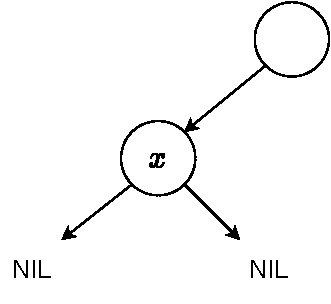
\includegraphics[scale=0.5]{img/del-leaf}
  \caption{Cut the leaf $x$ off.} \label{fig:del-leaf}
\end{figure}

\begin{figure}[htbp]
  \centering
  \subcaptionbox{Before delete $x$.}{\includegraphics[scale=0.5]{img/del-lc-before}}
  \subcaptionbox{After delete $x$, cut $x$ off, replace it with the left sub-tree.}{\includegraphics[scale=0.5]{img/del-lc-after}} \\
  \subcaptionbox{Before delete $x$.}{\includegraphics[scale=0.5]{img/del-rc-before}}
  \subcaptionbox{After delete $x$, cut $x$ off, replace it with the right sub-tree.}{\includegraphics[scale=0.5]{img/del-rc-after}}
  \caption{Delete a node with only a none empty sub-tree.}
  \label{fig:del-1child}
\end{figure}

\begin{figure}[htbp]
  \centering
  \subcaptionbox{Before delete $x$.}{\includegraphics[scale=0.5]{img/del-branch-before}}
  \subcaptionbox{After delete $x$, replace $x$ with the minimum from its right sub-tree.}{ \includegraphics[scale=0.5]{img/del-branch-after}}
  \caption{Delete a node with two none empty sub-trees.}
  \label{fig:del-branch}
\end{figure}

\be
\begin{array}{rcl}
delete\ x\ \nil & = & \nil\\
delete\ x\ (l, k, r) & = & \begin{cases}
  x < k: & (delete\ x l, k, r) \\
  x > k: & (l, k, delete\ x r) \\
  x = k: & del\ l\ r \\
\end{cases}
\end{array}
\ee

Where:

\be
\begin{array}{rcl}
del\ \nil\ r & = & r \\
del\ l\ \nil & = & l \\
del\ l\ r & = & (l, y, delete\ y\ r), y = \min\ r \\
\end{array}
\ee

The performance of delete is $O(h)$, where $h$ is the height of the tree. The imperative implementation needs set the parent reference in addition.

\begin{algorithmic}[1]
\Function{Delete}{$T, x$}
  \State $r \gets T$
  \State $x' \gets x$ \Comment{save $x$}
  \State $p \gets $ \Call{Parent}{$x$}
  \If{\Call{Left}{$x$} $= $ NIL}
    \State $x \gets $ \Call{Right}{$x$}
  \ElsIf{\Call{Right}{$x$} $= $ NIL}
    \State $x \gets $ \Call{Left}{$x$}
  \Else
    \Comment{neither sub-tree is empty}
    \State  $y \gets $ \textproc{Min}(\Call{Right}{$x$})
    \State \Call{Key}{$x$} $\gets$ \Call{Key}{$y$}
    \State \Call{Value}{$x$} $\gets$ \Call{Value}{$y$}
    \If{\Call{Parent}{$y$} $\neq x$}
      \Comment{$y$ does not have left sub-tree}
      \State \textproc{Left}(\Call{Parent}{$y$}) $\gets$ \Call{Right}{$y$}
    \Else
      \Comment{$y$ is the root of the right sub-tree}
      \State \Call{Right}{$x$} $\gets$ \Call{Right}{$y$}
    \EndIf
    \If{\Call{Right}{$y$} $\neq $ NIL}
      \State \textproc{Parent}(\Call{Right}{$y$}) $\gets$ \Call{Parent}{$y$}
    \EndIf
    \State Remove $y$
    \State \Return $r$
  \EndIf
  \If{$x \neq $ NIL}
    \State \Call{Parent}{$x$} $\gets p$
  \EndIf
  \If{$p = $ NIL}
    \Comment{remove the root}
    \State $r \gets x$
  \Else
    \If{\Call{Left}{$p$} $= x'$}
      \State \Call{Left}{$p$} $\gets x$
    \Else
      \State \Call{Right}{$p$} $\gets x$
    \EndIf
  \EndIf
  \State Remove $x'$
  \State \Return $r$
\EndFunction
\end{algorithmic}

Assume $x$ is not empty, first record the root, copy reference to $x$ and its parent. If either sub-tree is empty, then cut $x$ off. If neither sub-tree is empty, we locate the minimum node $y$ of the right sub-tree, replace the content of $x$ with $y$, then cut $y$ off. We also need handle the special case, that $y$ is the root of the right sub-tree. Finally, we need reset the stored parent if $x$ has only one none empty sub-tree. If the copied parent is empty, we are deleting the root. We return the new root in this case. After setting the parent, we can safely remove $x$. The deletion algorithm is bound to $O(h)$ time, where $h$ is the height of the tree.

\index{binary search tree!random build}
The performance of the binary search tree algorithms depends on the height $h$ of the tree. When unbalanced, $O(h)$ is close to $O(n)$, while for well balanced tree, $O(h)$ is close to $O(\lg n)$. Chapter 4 and 5 introduce self-balanced solution, there is another simple method to balance the tree: shuffle the elements, then build the tree\cite{CLRS}. It decreases the possibility of poorly balanced tree.

We can use binary search tree to realize the map data structure (also known as associative data structure or dictionary). A finite map is a collection of key-value pairs. Each key is unique, and is mapped to some value. For keys of type $K$, values of type $V$, the type of the map is $Map\ K\ V$ or \texttt{Map<K, V>}. For none empty map, it contains $n$ mappings of $\{k_1 \mapsto v_1, k_2 \mapsto v_2, ..., k_n \mapsto v_n\}$. When use the binary search tree to implement map, we constrain $K$ to be ordered set. Every node stores a pair of key and value. The type of the tree is $Tree\ (K, V)$. We use the tree insert/update operation to associate a key with a value. Given a key $k$, we use $lookup$ to find the mapped value $v$, or returns nothing or $\nil$ when $k$ does not exist. The red-black tree and AVL tree in chapter 4 and 5 can also implement map.

\begin{Exercise}\label{ex:bst-delete}
\Question{There is a symmetric deletion algorithm. When neither sub-tree is empty, we replace with the maximum of the left sub-tree, then cut the maximum off. Write a program to implement this solution.}
\Question{Write a randomly building algorithm for binary search tree.}
\Question{How to find the two nodes with the greatest distance in a binary tree?}
\end{Exercise}

\begin{Answer}[ref={ex:bst-delete}]
\Question{There is a symmetric deletion algorithm. When neither sub-tree is empty, we replace with the maximum of the left sub-tree, then cut the maximum off. Write a program to implement this solution.

\begin{Haskell}
delete _ Empty = Empty
delete x (Node l k r) | x < k = Node (delete x l) k r
                      | x > k = Node l k (delete x r)
                      | otherwise = del l r
  where
    del Empty r = r
    del l Empty = l
    del l r = let m = max l in Node (delete m l) m r
\end{Haskell}
}
\Question{Write a randomly building algorithm for binary search tree.

\begin{Haskell}
fromList = (foldr insert Empty) . shuffle
\end{Haskell}
}

\Question{How to find the two nodes with the greatest distance in a binary tree?

We first find the maximum distance $m$, then give the longest path $[s, a, b, ..., e]$. The two ends $s$ and $e$ are the two nodes in question. To define the distance between two nodes, let the connected path (without direction) be $s \to n_1 \to n_2 \to ... \to n_m \to e$, every edge has the length of 1, then the total length from $s$ to $e$ is the distance between them, which is $m + 1$. Define the maximum distance of the empty tree as 0. For singleton leaf $(\nil, k, \nil)$, as the longest path is $[k]$, the maximum distance is also 0 (from $k$ to $k$). Consider the branch node $(l, k, r)$, the maximum distance must be one of the three: (1) from the deepest node on the left to the root, then to the deepest node on the right: $depth\ l + depth\ r$; (2) the maximum distance of the left sub-tree $l$; (3) the maximum distance of the right sub-tree $r$.

\begin{Haskell}
maxDistance Empty = 0
maxDistance (Node Empty _ Empty) = 0
maxDistance (Node l _ r) = maximum [depth l + depth r,
                            maxDistance l, maxDistance r]
\end{Haskell}

Where the definition of $depth$ is in \cref{ex:bst-depth}. We can adjust it to find the longest path. For the empty tree, the longest path is $[\ ]$, for singleton leaf, the longest path is $[k]$, for branch node $(l, k, r)$, the longest path is the maximum of the three: (1) The reverse of the path from the root to the deepest node on the left, and $k$, and the path from the root the deepest node on the right; (2) the longest path of the left; (3) the longest path of the right.

\begin{Haskell}
maxPath Empty = []
maxPath (Node Empty k Empty) = [k]
maxPath (Node l k r) = longest [(reverse depthPath l) ++ k : depthPath r,
                         maxPath l, maxPath r] where
  longest = maximumBy (compare `on` length)
  depthPath = foldt id (\ xs k ys -> k : longest [xs, ys]) []
\end{Haskell}

This implementation traverse the tree when calculate the depth, then traverse another two rounds for the left and right sub-trees. To avoid duplication, we can bottom-up fill the depth $d$ and the maximum distance $m$ in each node. This can be done through tree map: $Tree\ A \mapsto Tree\ (Int, Int)$ in one traverse:

\begin{Haskell}
maxDist = extract . mapTr where
  extract Empty = 0
  extract (Node _ (_, m) _) = m
  mapTr Empty = Empty
  mapTr (Node l _ r) = f (mapTr l) (mapTr r)
  f l r = Node l (1 + max d1 d2, maximum [d1 + d2, m1, m2]) r where
    (d1, m1) = pairof l
    (d2, m2) = pairof r
    pairof Empty = (0, 0)
    pairof (Node _ k _) = k
\end{Haskell}

We can further simplify it with fold:

\begin{Haskell}
maxDist = snd . pair . foldt id g Empty where
  g l _ r = Node l (1 + max d1 d2, maximum [d1 + d2, m1, m2]) r where
    (d1, m1) = pair l
    (d2, m2) = pair r
  pair = (maybe (0, 0) id) . key
\end{Haskell}
}
\end{Answer}

\section{Appendix: Example programs}

Definition of binary search tree node with parent reference.

\lstset{language=Bourbaki, frame=single}
\begin{lstlisting}
data Node<T> {
    T key
    Node<T> left
    Node<T> right
    Node<T> parent

    Node(T k) = Node(null, k, null)

    Node(Node<T> l, T k, Node<T> r) {
        left = l, key = k, right = r
        if (left != null) then left.parent = this
        if (right != null) then right.parent = this
    }
}
\end{lstlisting}

Recursive insert without using pattern matching.

\begin{lstlisting}
Node<T> insert (Node<T> t, T x) {
    if (t == null) {
        return Node(null, x, null)
    } else if (t.key < x) {
        return Node(insert(t.left, x), t.key, t.right)
    } else {
        return Node(t.left, t.key, insert(t.right, x))
    }
}
\end{lstlisting}

Map and fold:

\begin{Haskell}
mapt _ Empty = Empty
mapt f (Node l x r)= Node (mapt f l) (f x) (mapt f r)

foldt _ _ z Empty = z
foldt f g z (Node l k r) = g (foldt f g z l) (f k) (foldt f g z r)

maptr :: (a -> b) -> Tree a -> Tree b
maptr f = foldt f Node Empty

fold _ z Empty = z
fold f z (Node l k r) = fold f (k `f` (fold f z r)) l
\end{Haskell}

Iterative lookup without recursion:

\begin{lstlisting}
Optional<Node<T>> lookup (Node<T> t, T x) {
    while (t != null and t.key != x) {
        if (x < t.key) {
            t = t.left
        } else {
            t = t.right
        }
    }
    return Optional.of(t);
}
\end{lstlisting}

Example iterative program to find the minimum of a tree.

\begin{lstlisting}
Optional<Node<T>> min (Node<T> t) {
    while (t != null and t.left != null) {
        t = t.left
    }
    return Optional.of(t);
}
\end{lstlisting}

Iterative find the successor.

\begin{lstlisting}
Optional<Node<T>> succ (Node<T> x) {
    if (x == null) {
        return Optional.Nothing
    } else if (x.right != null) {
        return min(x.right)
    } else {
        p = x.parent
        while (p != null and x == p.right) {
            x = p
            p = p.parent
        }
        return Optional.of(p);
    }
}
\end{lstlisting}

delete:

\begin{Haskell}
delete _ Empty = Empty
delete x (Node l k r) | x < k = Node (delete x l) k r
                      | x > k = Node l k (delete x r)
                      | otherwise = del l r
  where
    del Empty r = r
    del l Empty = l
    del l r = let k' = min r in Node l k' (delete k' r)
\end{Haskell}

\ifx\wholebook\relax \else
\section{Answers}
\shipoutAnswer

\begin{thebibliography}{99}

\bibitem{CLRS}
Thomas H. Cormen, Charles E. Leiserson, Ronald L. Rivest and Clifford Stein.
``Introduction to Algorithms, Second Edition''. ISBN:0262032937. The MIT Press. 2001

\bibitem{Bentley}
Jon Bentley. ``Programming Pearls(2nd Edition)''. Addison-Wesley Professional; 2 edition (October 7, 1999). ISBN-13: 978-0201657883

\bibitem{okasaki-blog}
Chris Okasaki. ``Ten Years of Purely Functional Data Structures''. \url{http://okasaki.blogspot.com/2008/02/ten-years-of-purely-functional-data.html}

\bibitem{sgi-stl}
SGI. ``Standard Template Library Programmer's Guide''. \url{http://www.sgi.com/tech/stl/}

\bibitem{literal-program}
\url{http://en.literateprograms.org/Category:Binary_search_tree}

\bibitem{wiki-fold}
\url{https://en.wikipedia.org/wiki/Foldl}

\bibitem{func-composition}
\url{https://en.wikipedia.org/wiki/Function_composition}

\bibitem{curry}
\url{https://en.wikipedia.org/wiki/Partial_application}

\bibitem{zipper-hbook}
Miran Lipovaca. ``Learn You a Haskell for Great Good! A Beginner's Guide''. the last chapter. No Starch Press; 1 edition April 2011, 400 pp. ISBN: 978-1-59327-283-8

\end{thebibliography}

\expandafter\enddocument
\fi
